\pdfoutput=1
\documentclass{article}


% if you need to pass options to natbib, use, e.g.:
%     \PassOptionsToPackage{numbers, compress}{natbib}
% before loading neurips_2024


% ready for submission
% \usepackage{neurips_2024}


% to compile a preprint version, e.g., for submission to arXiv, add add the
% [preprint] option:
\usepackage[preprint, nonatbib]{neurips_2024}

% to compile a camera-ready version, add the [final] option, e.g.:
%     \usepackage[final]{neurips_2024}


% to avoid loading the natbib package, add option nonatbib:
   % \usepackage[nonatbib]{neurips_2024}


\usepackage[utf8]{inputenc} % allow utf-8 input
\usepackage[T1]{fontenc}    % use 8-bit T1 fonts
\usepackage{hyperref}       % hyperlinks
\usepackage{url}            % simple URL typesetting
\usepackage{booktabs}       % professional-quality tables
\usepackage{amsfonts}       % blackboard math symbols
\usepackage{nicefrac}       % compact symbols for 1/2, etc.
\usepackage{microtype}      % microtypography
\usepackage{xcolor}         % colors

% include other package
\usepackage{colortbl}
\usepackage{graphicx}
\usepackage{multirow} 
\usepackage{amsmath}
\usepackage{mathrsfs}
\usepackage{subcaption}
\usepackage{cleveref}
\usepackage{amsfonts,amssymb}
% \usepackage{subfigure}
\usepackage{subcaption}
\usepackage{enumitem}

\title{SparseDrive: End-to-End Autonomous Driving via Sparse Scene Representation}


% The \author macro works with any number of authors. There are two commands
% used to separate the names and addresses of multiple authors: \And and \AND.
%
% Using \And between authors leaves it to LaTeX to determine where to break the
% lines. Using \AND forces a line break at that point. So, if LaTeX puts 3 of 4
% authors names on the first line, and the last on the second line, try using
% \AND instead of \And before the third author name.

\author{%
Wenchao Sun\textsuperscript{\textnormal{1,2}} \quad
Xuewu Lin\textsuperscript{\textnormal{2}} \quad
Yining Shi\textsuperscript{\textnormal{1}} \quad
Chuang Zhang\textsuperscript{\textnormal{1}} \quad 
Haoran Wu\textsuperscript{\textnormal{1}} \quad
Sifa Zheng\textsuperscript{\textnormal{1}}
\vspace{0.2cm}\\
$^1$ Tsinghua University \quad
$^2$ Horizon
}
% \author{%
%   Wenchao Sun\thanks{Use footnote for providing further information
%     about author (webpage, alternative address)---\emph{not} for acknowledging
%     funding agencies.} \\
%   School of Vehicle and Mobility\\
%   Tsinghua University\\
%   Pittsburgh, PA 15213 \\
%   \texttt{swc21@mails.tsinghua.edu.cn} \\
%   % examples of more authors
%   \And
%   Coauthor \\
%   Affiliation \\
%   Address \\
%   \texttt{email} \\
  % \AND
  % Coauthor \\
  % Affiliation \\
  % Address \\
  % \texttt{email} \\
  % \And
  % Coauthor \\
  % Affiliation \\
  % Address \\
  % \texttt{email} \\
  % \And
  % Coauthor \\
  % Affiliation \\
  % Address \\
  % \texttt{email} \\
% }

\begin{document}
\maketitle
\begin{abstract}
  
  Aligning Large Language Models (LLMs) traditionally relies on costly training and human preference annotations. Self-alignment seeks to reduce these expenses by enabling models to align themselves. To further lower costs and achieve alignment without any expensive tuning or annotations, we introduce a new tuning-free approach for self-alignment, Dynamic Rewarding with Prompt Optimization (\ours). Our approach leverages a search-based optimization framework that allows LLMs to iteratively self-improve and craft the optimal alignment instructions, all without additional training or human intervention. The core of \ours is a dynamic rewarding mechanism, which identifies and rectifies model-specific alignment weaknesses, allowing LLMs to adapt efficiently to diverse alignment challenges. Empirical evaluations on eight recent LLMs, both open- and closed-sourced, demonstrate that \ours significantly enhances alignment performance, with base models outperforming their SFT/RLHF-tuned counterparts. Moreover, the prompts automatically optimized by \ours surpass those curated by human experts, further validating the effectiveness of our approach. Our findings highlight the great potential of current LLMs to achieve adaptive self-alignment through inference-time optimization, complementing tuning-based alignment methods.\footnote{Code available: \url{https://github.com/Singla17/DRPO}}
  
\end{abstract}
\section{Introduction}
The advancement of reasoning models has significantly improved the mathematical capabilities of large language models (LLMs). Evaluation efforts like MathArena \citep{matharena} demonstrate that these models achieve impressive performance on mathematical competitions such as AIME and HMMT. However, these competitions only evaluate final numerical answers and do not require rigorous proof-based reasoning essential for most mathematical tasks. 

Current benchmarks that mitigate this issue either rely on formal verification tools like Lean \citep{minif2f,fimo,putnambench} or focus on the evaluation of constructive proofs \citep{mathconstruct}. While these approaches are useful, the former does not take advantage of LLMs' strong natural language generation capabilities, and the latter covers only a limited subset of proofs. Therefore, it remains uncertain whether LLMs can reliably address complex mathematical questions requiring rigorous reasoning, which are crucial in real-world mathematical contexts.

To overcome these limitations, we conduct the first evaluation of natural language proofs by LLMs on challenging problems from the 2025 USA Mathematical Olympiad (USAMO). The USAMO represents one of the highest tiers of high school mathematics competitions in the United States, demanding detailed proofs and explanations analogous to the International Mathematical Olympiad (IMO). Participants qualify through prior competitions, including the AIME, but USAMO problems require significantly more rigorous and well-explained solutions.

Overall, we find that current LLMs struggle significantly on USAMO problems, with the best-performing model achieving an average score of less than $25\%$. Our evaluation reveals several critical failure modes, including flawed logic, unjustified assumptions, and a lack of creativity in reasoning. These findings underscore the substantial limitations of current LLMs in generating rigorous mathematical proofs. In this report, we first outline our methodology in \cref{sec:meth}, present detailed results and identify critical weaknesses in \cref{sec:results}, and discuss several qualitative observations in \cref{sec:discussion}.


\section{Related Work}
\vspace{-5pt}


\noindent \textbf{Self-Alignment.}
Traditional alignment approaches rely heavily on extensive human-annotated preference data and complex reward model training through reinforcement learning, which poses significant scalability and cost challenges~\cite{ouyang2022training}. Self-alignment focuses on aligning LLMs themselves with model-generated feedback, datasets, critique, etc., which are then used for fine-tuning or training reward models~\cite{lee2023rlaif, bai2022training, cao2024towards, wang2024step, guo2024human}. Notable examples include synthesizing alignment training data with human-provided instructions and ICL examples~\cite{wang2022self, kim2023aligning, sun2024principle}, augmented web documents~\cite{li2023self}, or self-critique~\cite{bai2022constitutional, madaan2024self}. However, most of these methods still require an SFT/RLHF-tuning process to enhance alignment, along with some degree of human annotations or supervision. In contrast, \ours shares similar self-alignment principles using self-critique error feedback to gradually align the model, but it achieves this entirely without any model tuning or human supervision.



\begin{figure*}[ht]
    \centering
    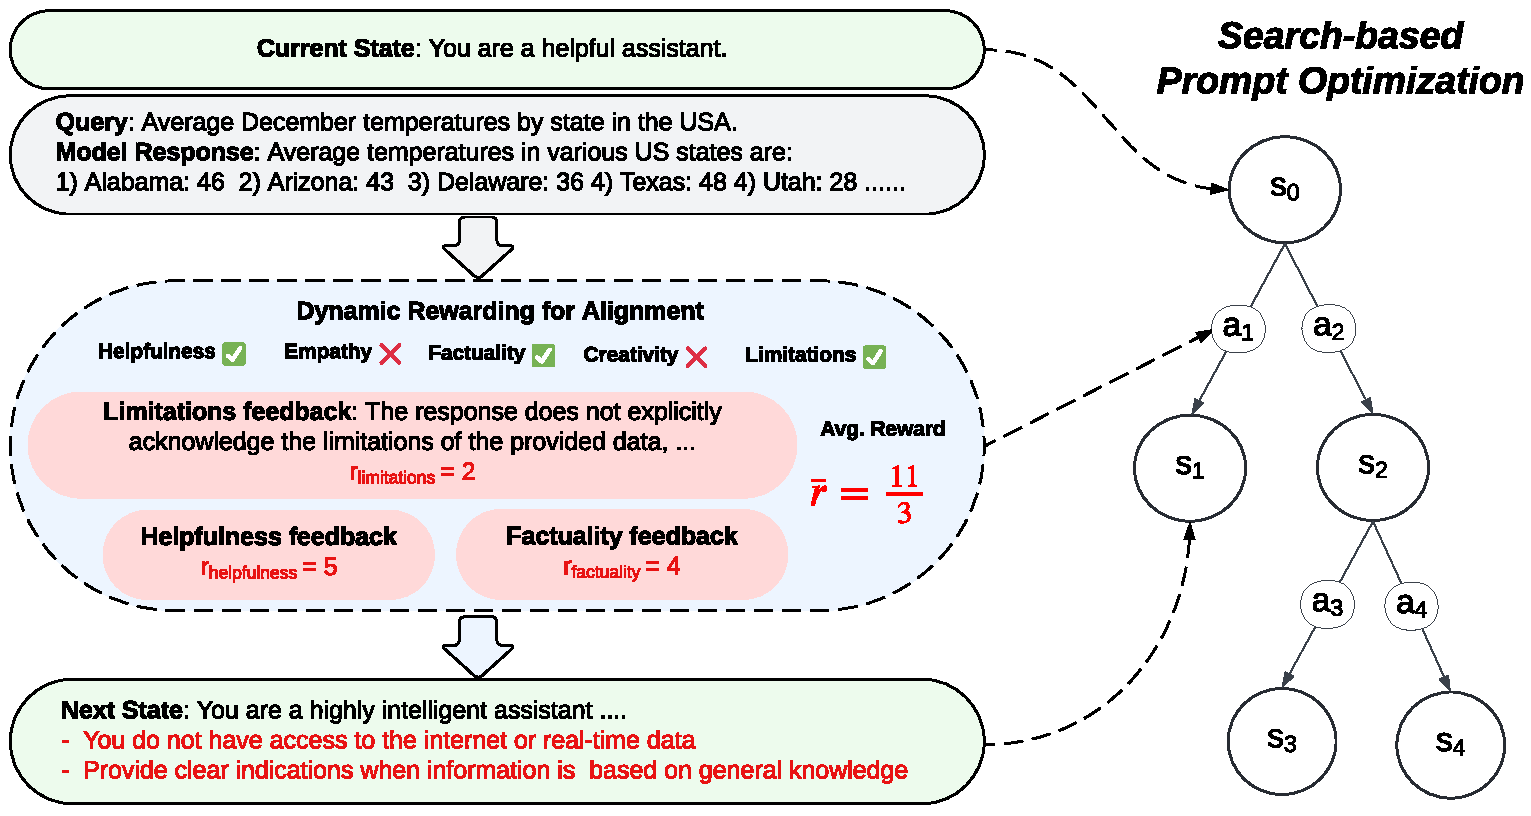
\includegraphics[width=0.95\linewidth]{images/Dynamic_Rewarding.pdf}
    \vspace{-8pt}
    \caption{Overall framework of Dynamic Rewarding with Prompt Optimization (\ours). The optimization problem is modeled as a Markov Decision Process (MDP) and solved using beam search to optimize the alignment prompt. Dynamic rewarding, a novel technique integrated into this framework, allows flexible reward assignment to detect and address alignment weaknesses in the current LLM, thereby enhancing the overall optimization process.
    }
    \label{fig:dynamic_rewarding}
    \vspace{-15pt}
\end{figure*}




\noindent \textbf{Tuning-Free Alignment.}
A recent trend in alignment research is to align LLMs without updating their parameters, typically as a post-training process for LLMs. This has witnessed two major lines of work recently. The first aligns models with carefully curated human annotations and ICL examples~\cite{han2023context, Lin2024ReAlign, zhao2024context}, while the second involves decoding-based methods to guide token generation and search with alignment rewards~\cite{li2023rain, khanov2024args, huang2024deal}. Although tuning-free, the first approach still requires human curation and often underperforms compared to SFT/RLHF-tuned counterparts. The second one, while effective, incurs higher inference costs per query, making it computationally expensive. It is worth mentioning that another recent promising direction is cost-efficient alignment through representation engineering~\cite{zou2023representation, wu2024reft}, which aims to steer LLM representation vectors for alignment~\cite{li2024inference, kong2024aligning, wang2024inferaligner}. However, these methods are not fully tuning-free and typically require additional data or model training to identify alignment directions in the embedding space. Nevertheless, \ours requires no additional annotations or model training, and also only needs a one-time optimization per model to achieve better performance than SFT/RLHF-tuned counterparts. 







\noindent \textbf{Prompt Optimization.}
Discovering optimal discrete prompts becomes far more crucial nowadays. Modern prompts for LLMs can be generally divided into two parts: in-context learning examples and detailed instructions. The former is usually treated as a retrieval problem with various schemas to select the influential examples~\cite{rubin2021learning, dong2022survey}. Optimizing the latter has been heavily studied recently, mostly formulated as a sampling or search problem. Generally, an initial prompt (e.g., a base prompt, ``You are a helpful assistant'') is given to start an iterative process, where diverse prompt candidates are generated per turn, and the best ones are kept for the next iteration. Various sampling strategies are proposed to diversify the prompt candidates, e.g., back translation~\cite{xu2022gps}, evolutionary operations~\cite{fernando2023promptbreeder}, self-critique~\cite{wang2023promptagent}. Different search frameworks also have been studied, such as Monte Carlo search~\cite{zhou2022large}, evolutionary algorithms~\cite{fernando2023promptbreeder, yang2023large}, beam search~\cite{pryzant2023automatic}, and Monte Carlo tree search (MCTS)~\cite{wang2023promptagent}. \ours builds upon recent search-based optimization methods but introduces novel techniques, such as dynamic rewarding, to effectively address the alignment problem. 
\begin{figure}[htbp]
  \centering
  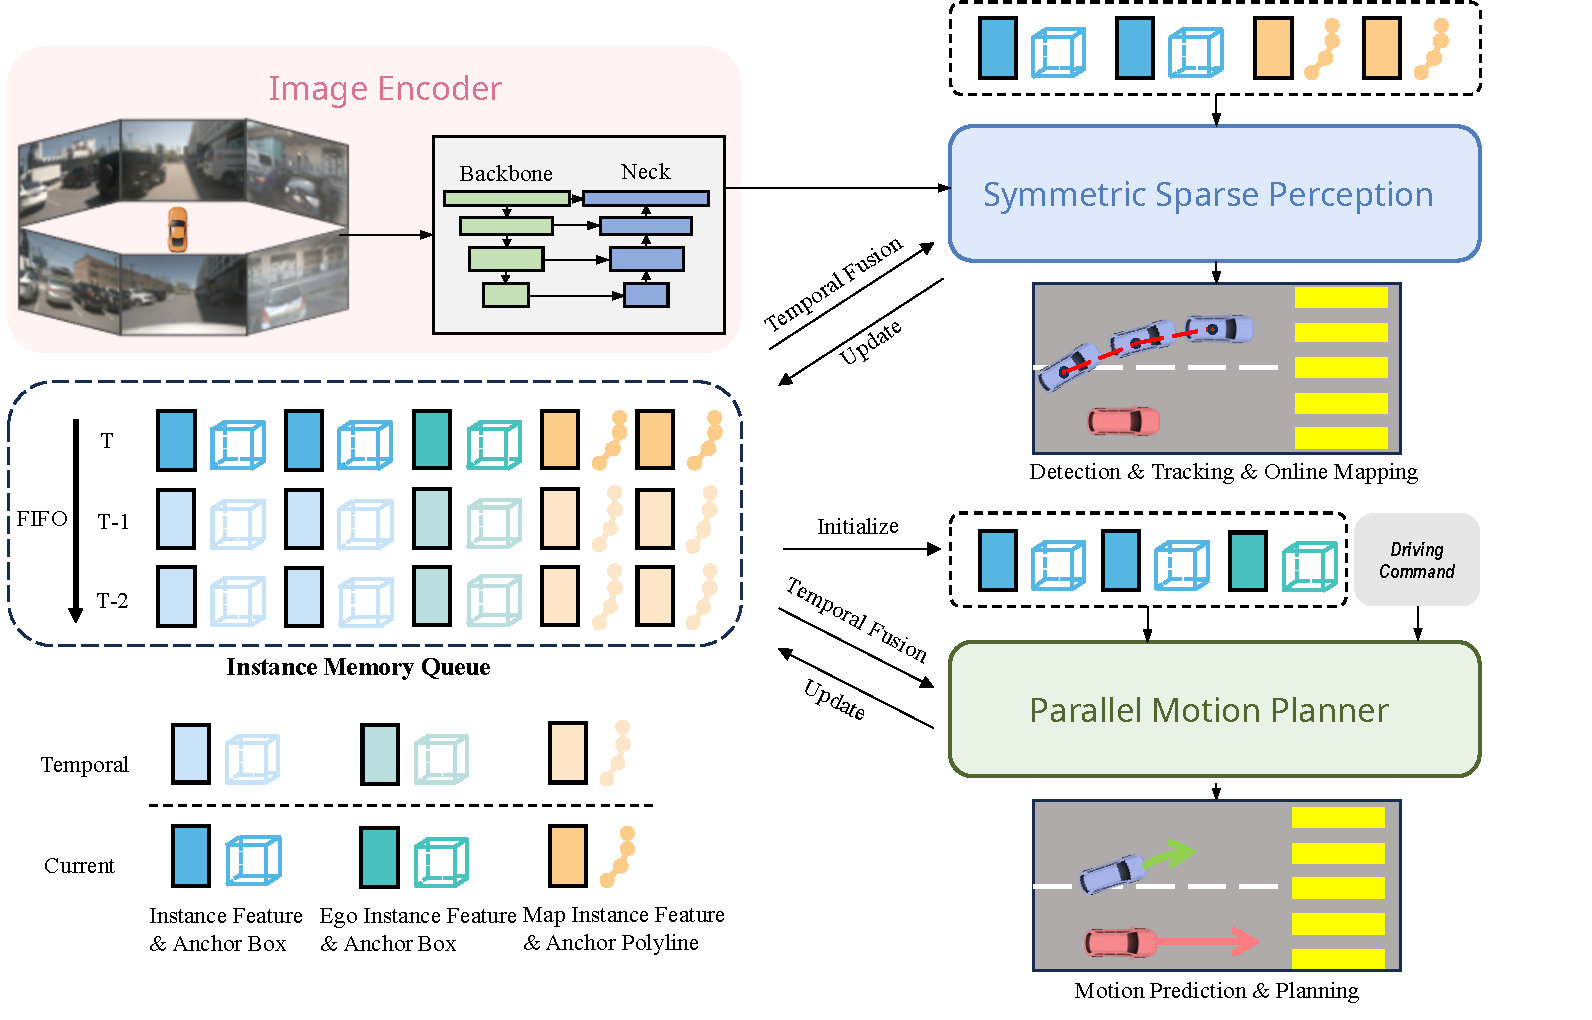
\includegraphics[width=0.8\linewidth]{Figures/overview_.pdf}
  \caption{Overview of SparseDrive. SparseDrive first encodes multi-view images into feature maps, then learns sparse scene representation through symmetric sparse perception, and finally perform motion prediction and planning in a parallel manner. An instance memory queue is devised for temporal modeling.}
  \label{fig:overview}
\end{figure}

\section{Method}
\subsection{Overview}
The overall framework of SparseDrive is depicted in Fig. \ref{fig:overview}. Specifically, SparseDrive is consisted of three parts: image encoder, symmetric sparse perception and parallel motion planner. Given multi-view images, the image encoder, including a backbone network and a neck, first encodes images to multi-view multi-scale feature maps $I=\left\{I_s \in \mathbb{R}^{N \times C \times H_s \times W_s} | 1 \leq s \leq S \right\}$, where $S$ is the number of scales and $N$ is the number of camera views. In symmetric sparse perception module, the feature maps $I$ are aggregated into two groups of instances to learn the sparse representation of the driving scene. These two groups of instances, representing surrounding agents and map elements respectively, are fed into parallel motion planner to interact with an initialized ego instance. The motion planner predicts multi-modal trajectories of surrounding agents and ego vehicle simultaneously, and selects a safe trajectory as the final planning result through hierarchical planning selection strategy.

\subsection{Symmetric Sparse Perception}
As shown in Fig. \ref{fig:sparse_perception}, the model structure of sparse perception module exhibits a structural symmetry, unifying detection, tracking and online mapping together.

\paragraph{Sparse Detection.}
Surrounding agents are represented by a group of instance features $F_d \in \mathbb{R}^{N_d \times C}$ and anchor boxes $B_d \in \mathbb{R}^{N_d \times 11}$, where $N_d$ is the number of anchors and $C$ is the feature channel dimension. Each anchor box is formatted  with location, dimension, yaw angle and velocity:
% \[ \left\{x,y,z,\mathrm{ln }w, \mathrm{ln}h, \mathrm{ln}l, \mathrm{sin}yaw, \mathrm{cos}yaw, vx, vy, vz\right\}. \]
\[ \left\{ x, y, z, \ln w, \ln h, \ln l, \sin{yaw}, \cos{yaw}, vx, vy, vz\right\}. \]

The sparse detection branch consists of $N_{dec}$ decoders, including a single non-temporal decoder and $N_{dec}-1$ temporal decoders. Each decoder takes feature maps $I$, instance features $F_d$ and anchor boxes $B_d$ as input, outputs updated instance features and refined anchor boxes. The non-temporal decoder takes randomly initialized instance as input, while the input for temporal decoder come from both current frame and historical frame. Specifically, the non-temporal decoder includes three sub-modules: deformable aggregation, feedforward network (FFN) and the output layer for refinement and classification. The deformable aggregation module generates fixed or learnable keypoints around the anchor boxes $B_d$ and projects them to feature maps $I$ for feature sampling. The instance features $F_d$ are updated by summation with sampled features, and are responsible for predicting the classification scores and the offsets of anchor boxes in the output layer. The temporal decoders have two additional multi-head attention layers: the temporal cross-attention between temporal instances from last frame and current instances, and the self-attention among current instances. In multi-head attention layer, the anchor boxes are transformed into high-dimensional anchor embedding $E_d \in \mathbb{R}^{N_d \times C}$, and serve as the positional encoding.

\begin{figure}[htbp]
  \centering
  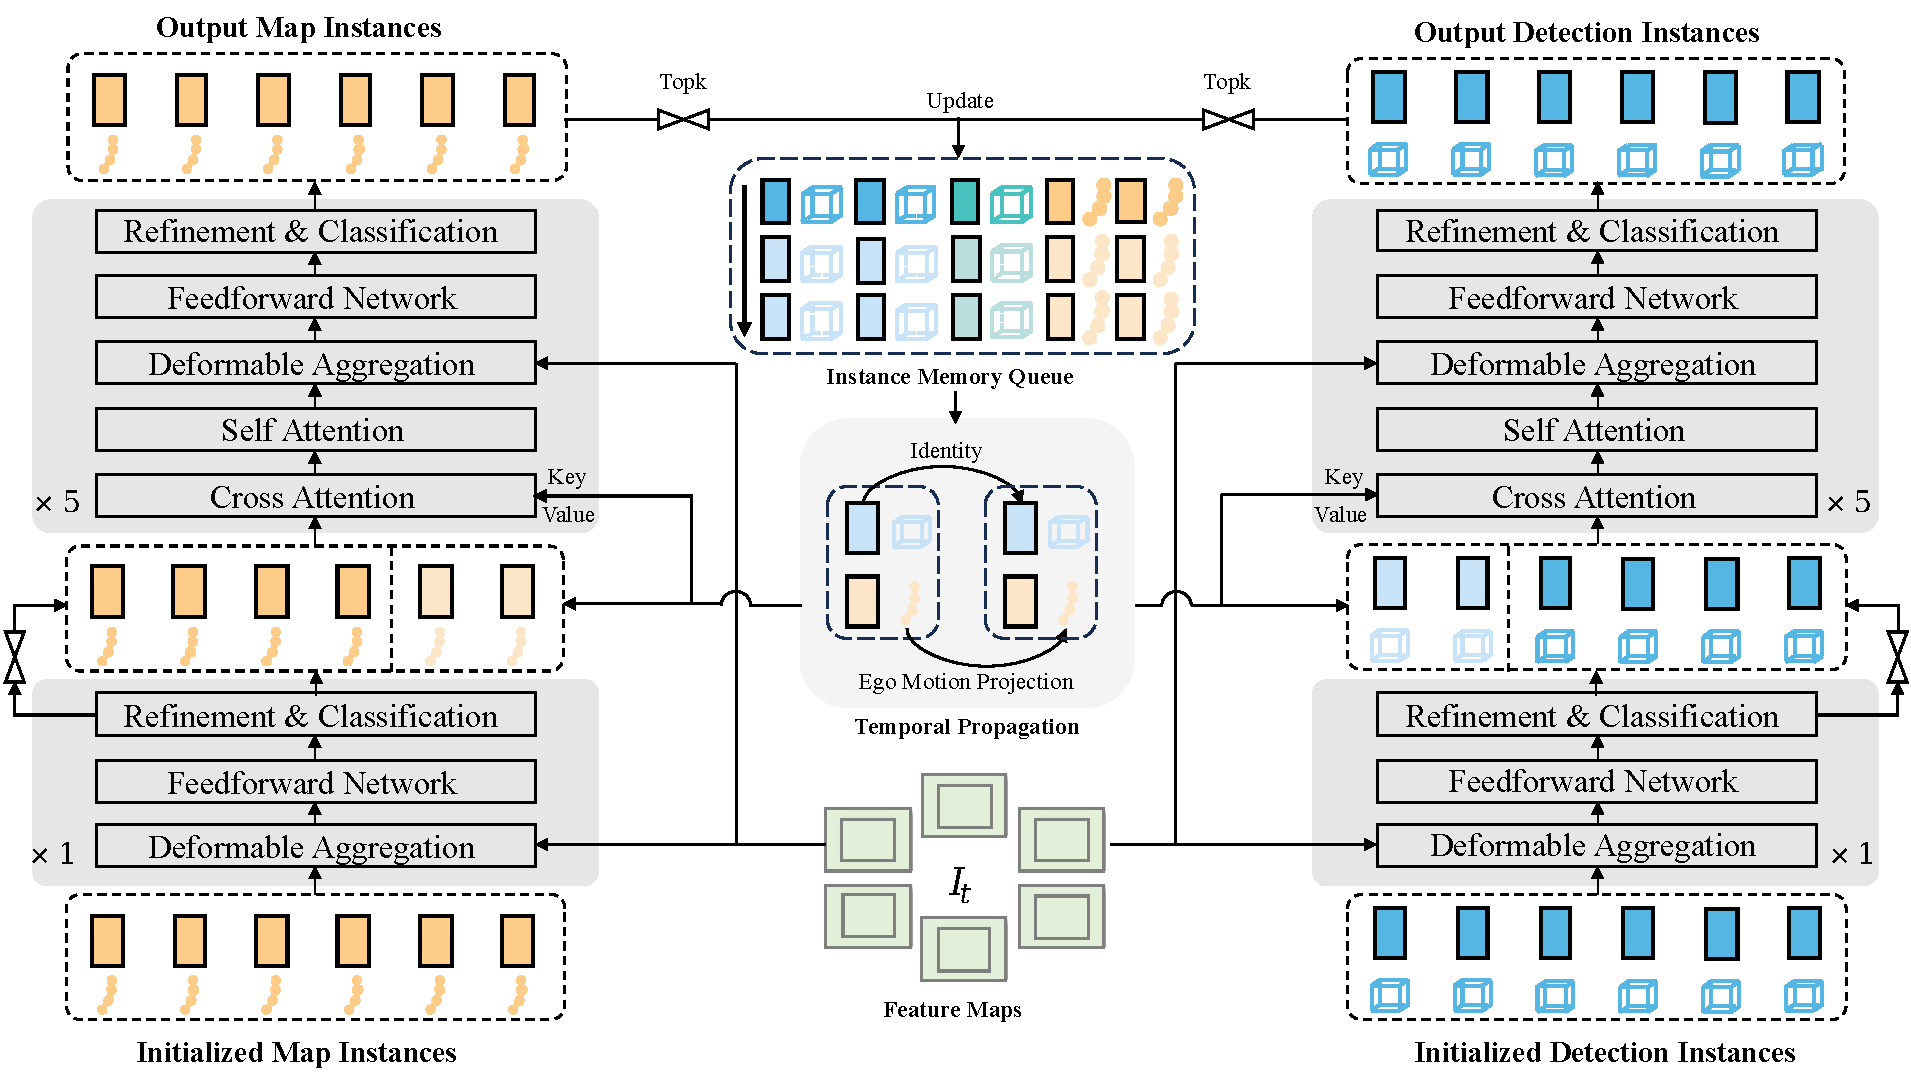
\includegraphics[width=0.85\linewidth]{Figures/sparse_perception_.pdf}
  \caption{Model architecture of symmetric sparse perception, which unifies detection, tracking and online mapping in a symmetric structure.}
  \label{fig:sparse_perception}
\end{figure}

\paragraph{Sparse Online Mapping.}
Online mapping branch shares the same model structure with detection branch except different instance definition. For static map element, the anchor is formulated as a polyline with $N_p$ points: \[ \left\{x_{0},y_{0},x_{1},y_{1},...,x_{N_p-1},y_{N_p-1} \right\}. \] 

Then all the map elements can be represented by map instance features $F_m \in \mathbb{R}^{N_m \times C}$ and anchor polylines $L_m \in \mathbb{R}^{N_m \times N_p \times 2}$, where $N_m$ is the number of anchor polylines.

\paragraph{Sparse Tracking.}
For tracking, we follow the ID assignment process of Sparse4Dv3\cite{sparse4dv3}: once the detection confidence of an instance surpasses a threshold $T_{thresh}$, it is locked onto a target and assigned with an ID, which remains unchanged throughout temporal propagation. This tracking strategy does not need any tracking constraints, resulting in an elegant and simple symmetric design for sparse perception module.

\subsection{Parallel Motion Planner}
As shown in Fig. \ref{fig:motion_planner}, the parallel motion planner consists of three parts: ego instance initialization, spatial-temporal interactions and hierarchical planning selection.

\paragraph{Ego Instance Initialization.}
Similar to surrounding agents, ego vehicle is represented by ego instance feature $F_e \in \mathbb{R}^{1 \times C}$  and ego anchor box $B_e \in \mathbb{R}^{1 \times 11}$. While ego feature is typically randomly initialized in previous methods, we argue that the ego feature also requires rich semantic and geometric information for planning, similar to motion prediction. However, the instance features of surrounding agents are aggregated from image feature maps $I$, which is not feasible for ego vehicle, since ego vehicle is in blind area of cameras. Thus we use the smallest feature map of front camera to initialize the ego instance feature: 
\begin{equation}
F_e = {\rm AveragePool}(I_{front,S})
\end{equation}
There are two advantages in doing so: the smallest feature map has already encoded the semantic context of the driving scene, and the dense feature map serves as a complementary for sparse scene representation, in case there are some blacklist obstacles, which can not be detected in sparse perception.

For ego anchor $B_e$, the location, dimension and yaw angle can be naturally set, as we are aware of these information of ego vehicle. For velocity, directly initialized from ground truth velocity leads to ego status leakage, as illustrated in \cite{ego}. So we add an auxiliary task to decode current ego status $ES_T$, including velocity, acceleration, angular velocity and steering angle. At each frame, we use the predicted velocity from last frame as the initialization of ego anchor velocity.

\begin{figure}[htbp]
  \centering
  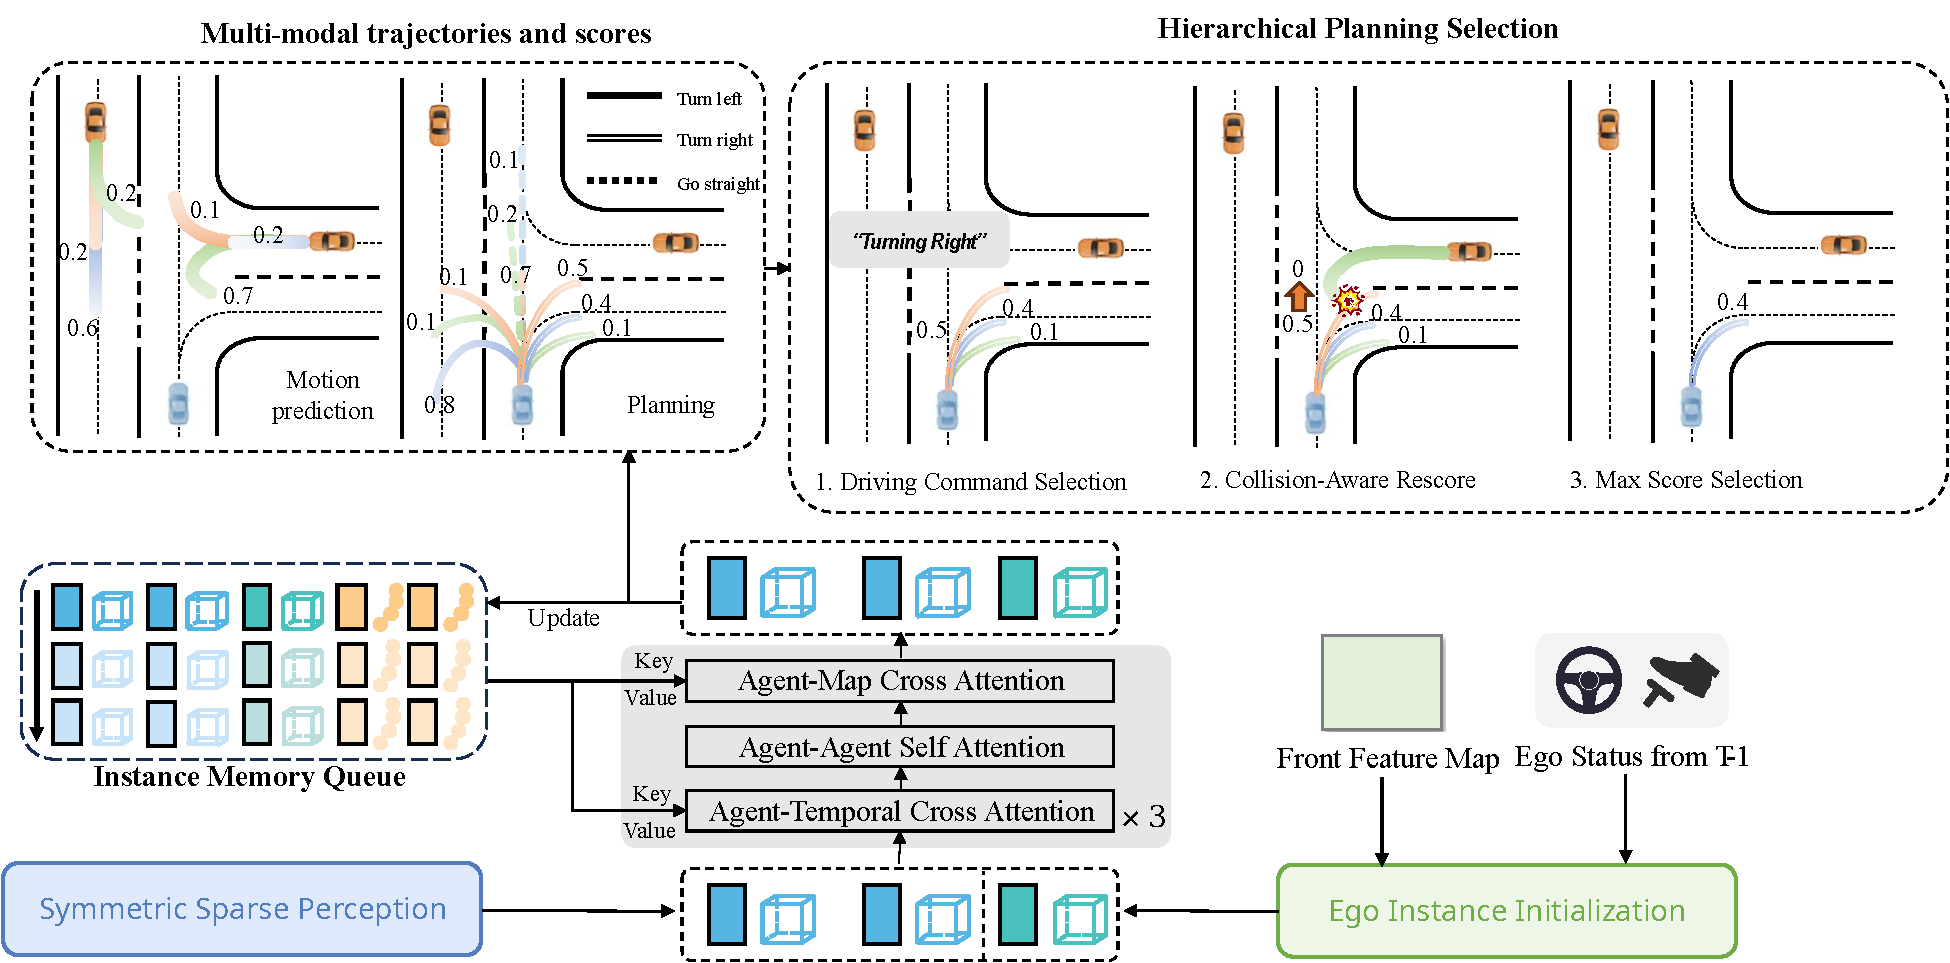
\includegraphics[width=0.83\linewidth]{Figures/motion_planner_.pdf}
  \caption{Model structure of parallel motion planner, which performs motion prediction and planning simultaneously and outputs safe planning trajectory.}
  \label{fig:motion_planner}
\end{figure}

\paragraph{Spatial-Temporal Interactions.}
To consider the high-level interaction between all road agents, we concatenate the ego instance with surrounding agents to get agent-level instances:
\begin{equation}
F_a={\rm Concat}(F_d, F_e), B_a={\rm Concat}(B_d, B_e)
\end{equation}
As the ego instance is initialized without temporal cues, which is important for planning, we devise an instance memory queue with the size of $(N_d+1) \times H$ for temporal modeling, $H$ is the number of stored frames. Then three types of interactions are performed to aggregate spatial-temporal context: agent-temporal cross-attention, agent-agent self-attention and agent-map cross-attention. Note that in temporal cross-attention of sparse perception module, the instances of current frame interact with all temporal instances, which we name as scene-level interaction. While for agent-temporal cross-attention here, we adopt instance-level interaction to make each instance focus on history information of itself.

Then, we predict the multi-modal trajectories $\tau_m \in \mathbb{R}^{N_{d} \times \mathcal{K}_m \times T_{m} \times 2}$, $\tau_p \in \mathbb{R}^{N_{c} \times \mathcal{K}_p \times T_{p} \times 2 }$ and scores $s_m \in \mathbb{R}^{N_{d} \times \mathcal{K}_m}$, $s_p \in \mathbb{R}^{N_{cmd} \times \mathcal{K}_p}$ for both surrounding agents and ego vehicle, $\mathcal{K}_m$ and $\mathcal{K}_p$ are the number of modes for motion prediction and planning, $T_m$ and $T_p$ are the number of future timestamps for motion prediction and planning, and $N_{cmd}$ is the number of driving command for planning. Following the common practice\cite{uniad, vad}, we use three kinds of driving commands: turn left, turn right and go straight. For planning, we additionally predict current ego status from ego instance feature.

\paragraph{Hierarchical Planning Selection.}
Now we have the multi-modal planning trajectory proposals, to select one safe trajectory $\tau_p^* $ to follow, we design a hierarchical planning selection strategy. First, we select a subset of trajectory proposals $\tau_{p,cmd} \in \mathcal{K}_p \times T_{p} \times 2$, corresponding to the high-level command $cmd$. Then, a novel collision-aware rescore module is adopted to ensure safety. With the motion prediction results, we can assess the collision risk of each planning trajectory proposal, for the trajectory with high collision probability, we reduce the score of this trajectory. In practice, we simply set the score of collided trajectory to $0$. Finally, we select the trajectory with the highest score as the final planning output.

\subsection{End-to-End Learning}
\paragraph{Multi-stage Training.}
The training of SparseDrive is divided into two stages. In stage-1, we train symmetric sparse perception module from scratch to learn the sparse scene representation. In stage-2, sparse perception module and parallel motion planner are trained together with no model weights frozen, fully enjoying the benefit of end-to-end optimization. More training details are provided in Appendix \ref{app:training}.

\paragraph{Loss Functions.}
The loss functions include the loss of four tasks, and the loss of each task can be further divider into classification loss and regression loss. For multi-modal motion prediction and planning task, we adopt the winner-takes-all strategy. For planning, there is an additional regression loss for ego status. We also introduce depth estimation as an auxiliary task to enhance the training stability of the perception module. The overall loss function for end-to-end training is: 
\begin{equation}
\mathcal{L}=\mathcal{L}_{det}+\mathcal{L}_{map}+\mathcal{L}_{motion}+\mathcal{L}_{plan}+\mathcal{L}_{depth}.
\end{equation}
More details about loss functions are provided in Appendix \ref{app:loss_func}.


\section{Experiments} \label{experiments}
Our experiments are conducted on challenging nuScenes\cite{nuscenes} dataset, which contains 1000 complex driving scenes, and each lasts for about 20 seconds. Evaluation metrics of each task are described in Appendix \ref{app:metric}. We have two variants of the model, which only differ in backbone network and input image resolution. For our small model SparseDrive-S, we use ResNet50\cite{resnet} as backbone network and the input image size is 256$\times$704. For our base model, SparseDrive-B, we change backbone network to ResNet101 and input image size to 512$\times$1408. All experiments are conducted on 8 NVIDIA RTX 4090 24GB GPUs. More configuration details are provided in Appendix \ref{app:imp_detail}.

\subsection{Main Results}
We compare with prior state-of-the-arts, both modularized and end-to-end methods. Among end-to-end methods, our lightweight model SparseDrive-S has surpassed previous SOTAs in all tasks, while our base model SparseDrive-B pushes the performance boundaries one step further. The main metrics for each task are marked in grey background in Tables.

\paragraph{Perception.} For 3D detection in Tab. \ref{tab:detection}, SparseDrive achieves \textbf{49.6\%} mAP and \textbf{58.8\%} NDS, yielding a significant improvement of \textbf{+11.6\%} mAP and \textbf{+9.0\%} NDS compared to UniAD\cite{uniad}. For multi-object tracking in Tab. \ref{tab:tracking}, SparseDrive achieves \textbf{50.1\%} AMOTA, and lowest ID switch of \textbf{632}, which surpasses UniAD\cite{uniad} by \textbf{+14.2\%} in terms of AMOTA and gets a \textbf{30.2\%} reduction for ID switch, showing the temporal consistency of tracking tracklet. For online mapping in Tab. \ref{tab:online_mapping}, SparseDrive gets a mAP of \textbf{56.2\%}, also surpassing previous end-to-end method VAD\cite{vad} by \textbf{+8.6\%}.

\begin{table}[t]
\caption{Perception results on nuScenes val dataset. SparseDrive achieves best perfomance on all perception tasks among end-to-end methods. $\dagger$: Reproduced with offcial checkpoint.}
\vspace{5pt}
\begin{subtable}[h]{1.0\textwidth}
\centering
% \resizebox{0.95\linewidth}{!}
\scriptsize
{
% \setlength{\tabcolsep}{4.0mm}
\begin{tabular}{l|c|c|ccccc|c}
\toprule
Method & Backbone & mAP$\uparrow$ & mATE$\downarrow$ & mASE$\downarrow$ & mAOE$\downarrow$ & mAVE$\downarrow$ & mAAE$\downarrow$ & \cellcolor{gray!30}NDS$\uparrow$ \\
\midrule
UniAD$^\dagger$~\cite{uniad} & ResNet101 & 0.380 & 0.684 & 0.277 & 0.383 & 0.381 & 0.192 & \cellcolor{gray!30}0.498 \\
SparseDrive-S & ResNet50 & 0.418 & 0.566 & 0.275 & 0.552 & 0.261 & 0.190 & \cellcolor{gray!30}0.525 \\
SparseDrive-B & ResNet101 & \textbf{0.496} & \textbf{0.543} & \textbf{0.269} & \textbf{0.376} & \textbf{0.229} & \textbf{0.179} & \cellcolor{gray!30}\textbf{0.588} \\
\bottomrule
\end{tabular}
}
\caption{3D detection results.}
\label{tab:detection}
\end{subtable}
\begin{subtable}[h]{1.0\textwidth}
\begin{subtable}[h]{0.45\textwidth}
\centering
% \resizebox{0.90\linewidth}{!}
\scriptsize
{
\setlength{\tabcolsep}{0.8mm}
\begin{tabular}{l|cccc}
\toprule
Method & \cellcolor{gray!30}AMOTA$\uparrow$ & AMOTP$\downarrow$ & Recall$\uparrow$ & IDS$\downarrow$ \\
\midrule
ViP3D~\cite{vip3d} & \cellcolor{gray!30}0.217 & 1.625 & 0.363 & - \\
QD3DT~\cite{qd3dt} & \cellcolor{gray!30}0.242 & 1.518 & 0.399 & - \\
MUTR3D~\cite{mutr3d} & \cellcolor{gray!30}0.294 & 1.498 & 0.427 & 3822 \\
\midrule
UniAD~\cite{uniad} & \cellcolor{gray!30}0.359 & 1.320 & 0.467 & 906 \\
SparseDrive-S & \cellcolor{gray!30}0.386 & 1.254 & 0.499 & 886 \\
SparseDrive-B & \cellcolor{gray!30}\textbf{0.501} & \textbf{1.085} & \textbf{0.601} & \textbf{632} \\
\bottomrule
\end{tabular}
}
\caption{Multi-object tracking results.}
\label{tab:tracking}
\end{subtable}
\hfill
\begin{subtable}[h]{0.55\textwidth}
% \resizebox{0.92\linewidth}{!}
\scriptsize
{
\setlength{\tabcolsep}{0.6mm}
\begin{tabular}{l|ccc|c}
\toprule
Method & $AP_{ped}\uparrow$ & $AP_{divider}\uparrow$ & $AP_{boundry}\uparrow$ & \cellcolor{gray!30}mAP$\uparrow$ \\
\midrule
HDMapNet~\cite{hdmapnet} & 14.4 & 21.7 & 33.0 & \cellcolor{gray!30}23.0 \\
VectorMapNet~\cite{vectormapnet} & 36.1 & 47.3 & 39.3 & \cellcolor{gray!30}40.9 \\
MapTR~\cite{maptr} & \textbf{56.2} & \textbf{59.8} & \textbf{60.1} & \cellcolor{gray!30}\textbf{58.7} \\
\midrule
% VAD-Tiny & 31.7 & 42.2 & 45.6 & 39.8 \\
VAD$^\dagger$~\cite{vad} & 40.6 & 51.5 & 50.6 & \cellcolor{gray!30}47.6 \\
SparseDrive-S & 49.9 & \textbf{57.0} & 58.4 & \cellcolor{gray!30}55.1 \\
SparseDrive-B & \textbf{53.2} & 56.3 & \textbf{59.1} & \cellcolor{gray!30}\textbf{56.2} \\
\bottomrule
\end{tabular}
}
\caption{Online mapping results.}
\label{tab:online_mapping}
\end{subtable}
\end{subtable}
\end{table}

\paragraph{Prediction.} For motion prediction in Tab. \ref{tab:motion}, SparseDrive achieves the best performance with \textbf{0.60m} minADE, \textbf{0.96m} minFDE, \textbf{13.2\%} MissRate and \textbf{0.555} EPA. Compared with UniAD\cite{uniad}, SparseDrive reduces errors by \textbf{15.5\%} and \textbf{5.9\%} on minADE and minFDE respectively.

\paragraph{Planning.} For planning in Tab. \ref{tab:planning}, among all methods, SparseDrive achieves a remarkable planning performance, with the lowest L2 error of \textbf{0.58m} and collision rate of \textbf{0.06\%}. Compared with previous SOTA VAD\cite{vad}, SparseDrive reduces L2 error by \textbf{19.4\%} and collision rate by \textbf{71.4\%}, demonstrating the effectiveness and safety of our method. 

\paragraph{Efficiency.} As shown in Tab. \ref{tab:efficiency}, besides the excellent performance, SparseDrive also achieves much higher efficiency for both training and inference. With the same backbone network, our base model achieves \textbf{4.8$\times$} faster in training and \textbf{4.1$\times$} faster in inference, compared with UniAD\cite{uniad}. Our lightweight model can achieve \textbf{7.2 $\times$} and \textbf{5.0$\times$} faster in training and inference. \textbf{}

\begin{table}[t]
\caption{Motion prediction and planning results on nuScenes val dataset. SparseDrive outperforms previous methods by a large margin. $\dagger$: Reproduced with offcial checkpoint. $^*$: LiDAR-based methods.}
\vspace{5pt}
\begin{subtable}[h]{0.4\textwidth}
\centering
\scriptsize
{
\setlength{\tabcolsep}{0.8mm}
\begin{tabular}{l|cccc}
\toprule
Method & \cellcolor{gray!30}minADE($m$)$\downarrow$ & minFDE($m$)$\downarrow$ & MR$\downarrow$ & EPA$\uparrow$  \\
\midrule
Cons Pos.~\cite{uniad} & \cellcolor{gray!30}5.80 & 10.27 & 0.347 & - \\
Cons Vel.~\cite{uniad} & \cellcolor{gray!30}2.13 & 4.01 & 0.318 & - \\
Traditional~\cite{vip3d} & \cellcolor{gray!30}2.06 & 3.02 & 0.277 & 0.209 \\
PnPNet~\cite{pnpnet} & \cellcolor{gray!30}1.15 & 1.95 & 0.226 & 0.222 \\
ViP3D~\cite{vip3d} & \cellcolor{gray!30}2.05 & 2.84 & 0.246 & 0.226 \\
\midrule
UniAD\cite{uniad} & \cellcolor{gray!30}0.71 & 1.02 & 0.151 & 0.456 \\
SparseDrive-S & \cellcolor{gray!30}0.62 & 0.99 & 0.136 & 0.482 \\
SparseDrive-B & \cellcolor{gray!30}\textbf{0.60} & \textbf{0.96} & \textbf{0.132} & \textbf{0.555} \\
\bottomrule
\end{tabular}
}
\caption{Prediction results.}
\label{tab:motion}
\end{subtable}
\hfill
\begin{subtable}[h]{0.6\textwidth}
\centering
\scriptsize
{
\setlength{\tabcolsep}{0.8mm}
\begin{tabular}{l|cccc|cccc}
\toprule
\multirow{2}{*}{Method} &
\multicolumn{4}{c|}{L2($m$)$\downarrow$} & 
\multicolumn{4}{c}{Col. Rate(\%)$\downarrow$} \\
& 1$s$ & 2$s$ & 3$s$ & \cellcolor{gray!30}Avg. & 1$s$ & 2$s$ & 3$s$ & \cellcolor{gray!30}Avg.\\
\midrule
FF$^*$~\cite{ff} & 0.55 & 1.20 & 2.54 & \cellcolor{gray!30}1.43 & 0.06 & 0.17 & 1.07 & \cellcolor{gray!30}0.43 \\
EO$^*$~\cite{eo} & 0.67 & 1.36 & 2.78 & \cellcolor{gray!30}1.60 & 0.04 & 0.09 & 0.88 & \cellcolor{gray!30}0.33 \\
\midrule
ST-P3~\cite{stp3} & 1.33 & 2.11 & 2.90 & \cellcolor{gray!30}2.11 & 0.23 & 0.62 & 1.27 & \cellcolor{gray!30}0.71 \\
UniAD$^\dagger$~\cite{uniad} & 0.45 & 0.70 & 1.04 & \cellcolor{gray!30}0.73 & 0.62 & 0.58 & 0.63  & \cellcolor{gray!30}0.61 \\
VAD$^\dagger$~\cite{vad} & 0.41 & 0.70 & 1.05 & \cellcolor{gray!30}0.72 & 0.03 & 0.19 & 0.43  & \cellcolor{gray!30}0.21 \\ 
SparseDrive-S & \textbf{0.29} & 0.58 & 0.96 & \cellcolor{gray!30}0.61 & \textbf{0.01} & 0.05 & 0.18 & \cellcolor{gray!30}0.08 \\
SparseDrive-B &\textbf{0.29} & \textbf{0.55} & \textbf{0.91} & \cellcolor{gray!30}\textbf{0.58} & \textbf{0.01} & \textbf{0.02} & \textbf{0.13} & \cellcolor{gray!30}\textbf{0.06} \\
\bottomrule
\end{tabular}
}
\caption{Planning results.}
\label{tab:planning}
\end{subtable}
\end{table}

\begin{table}[htbp]
\centering
\caption{Efficiency comparison results. SparseDrive achieves high efficiency for both training and inference. Training time and FPS for UniAD are measured on 8 and 1 NVIDIA Tesla A100 GPUs respectively. Training time and FPS for SparseDrive are measured on 8 and 1 NVIDIA Geforce RTX 4090 GPUs respectively.}
\label{tab:efficiency}
\vspace{5pt}
\resizebox{0.90\linewidth}{!}
{    
\begin{tabular}{c|ccc|cccc}
\toprule
\multirow{2}{*}{Method} &
\multicolumn{3}{c|}{Training Efficiency} & 
\multicolumn{4}{c}{Inference Efficiency} \\
& GPU Memory (G) & Batch Size & Time (h) & GPU Memory (M) & FLOPs (G) & Params (M) & FPS\\
\midrule
UniAD~\cite{uniad} & 50.0 & 1 & 48 + 96 & 2451 & 1709 & 125.0 & 1.8 \\
\midrule
SparseDrive-S & 15.2 & 6 & 18 + 2 & 1294 & 192 & 85.9 & 9.0 \\
SparseDrive-B & 17.6 & 4 & 26 + 4 & 1437 & 787 & 104.7 & 7.3 \\
\bottomrule
\end{tabular}
}
\end{table} 

\subsection{Ablation Study}
We conduct extensive ablation studies to demonstrate the effectiveness of our design choices. We use SparseDrive-S as the default model for ablation experiments.

\paragraph{Effect of designs in Motion Planner.}
To underscore the significance of considering similarity between prediction and planning, we devised several specific experiments, as shown in Tab. \ref{tab:ablation_motion_planner}. ID-2 ignores the impact of ego vehicle on surrounding agents by changing the parallel design for prediction and planning to sequential order, leading to worse performance for motion prediction and collision rate. ID-3 randomly initializes ego instance feature and set all parameters of ego anchor to 0. Removing the semantic and geometric information of ego instance leads to performance degradation in both L2 error and collision rate. ID-4 takes planning as a deterministic problem and only outputs one certain trajectory, resulting in highest collision rate. Moreover, ID-5 removes the instance-level agent-temporal cross-attention, seriously degrading the L2 error to 0.77m. For collision-aware rescore, we have detailed discussion in the following paragraph.

\paragraph{Collision-Aware Rescore.} In previous methods\cite{uniad, graphad}, a post-optimization strategy is adopted to ensure safety based on perception results. However, we argue that this strategy breaks the end-to-end paradigm, resulting in serious degradation in L2 error, as shown in Tab. \ref{tab:ablation_CAR}. Moreover, under our re-implemented collision rate metric, the post-optimization does not make planning safer, but rather more dangerous. By contrast, our collision-aware rescore module reduces collision rate from 0.12\% to 0.08\%, with negligible increase in L2 error, showing the superiority of our method.

\paragraph{Multi-modal planning.}
We conduct experiments on the number of planning modes. As shown in Tab. \ref{tab:ablation_planning_mode}, with the number of planning modes increases, the planning performance improves continuously until saturated at 6 modes, again proving the importance of multi-modal planning.

\begin{table}[htbp]
\centering
\caption{Ablation for designs in parallel motion planner. "PAL" means parallel design for motion prediction and planning task; "EII" means ego instance initialization; "MTM" means multiple mode for planning; "ATA" means agent-temporal cross-attention; "CAR" means collision-aware rescore.}
\label{tab:ablation_motion_planner}
\vspace{5pt}
% \resizebox{0.90\linewidth}{!}
\scriptsize
{    
\setlength{\tabcolsep}{1.5mm}
\begin{tabular}{l|ccccc|ccc|cccc|cccc}
\toprule
\multirow{2}{*}{ID} &
\multirow{2}{*}{PAL} & 
\multirow{2}{*}{EII} & 
\multirow{2}{*}{MTM} &
\multirow{2}{*}{ATA} & 
\multirow{2}{*}{CAR} &
\multicolumn{3}{c|}{Prediction} & 
\multicolumn{4}{c|}{Planning L2($m$)} & 
\multicolumn{4}{c}{Planning Coll.(\%)} \\
&&&&&& \cellcolor{gray!30}minADE & minFDE & MR & 1$s$ & 2$s$ & 3$s$ & \cellcolor{gray!30}Avg. & 1$s$ & 2$s$ & 3$s$ & \cellcolor{gray!30}Avg.\\
\midrule
1 & \checkmark & \checkmark & \checkmark & \checkmark & \checkmark & \cellcolor{gray!30}0.623 & \textbf{0.987} & 0.136 & \textbf{0.29} & \textbf{0.58} & 0.96 & \cellcolor{gray!30}\textbf{0.61} & \textbf{0.01} & \textbf{0.05} & \textbf{0.18} & \cellcolor{gray!30}\textbf{0.08} \\
2 & & \checkmark & \checkmark & \checkmark & \checkmark & \cellcolor{gray!30}0.641 & 1.008 & 0.138 & 0.30 & 0.58 & 0.95 & \cellcolor{gray!30}\textbf{0.61} & 0.02 & 0.06 & 0.23 & \cellcolor{gray!30}0.10\\
3 & \checkmark &  & \checkmark & \checkmark & \checkmark & \cellcolor{gray!30}\textbf{0.621} & 0.988 & \textbf{0.135} & 0.31 & 0.60 & 0.98 & \cellcolor{gray!30}0.63 & 0.03 & 0.07 & 0.21 &  \cellcolor{gray!30}0.11\\
4 & \checkmark & \checkmark & & \checkmark & \checkmark & \cellcolor{gray!30}0.626 & 1.002 & 0.136 & 0.33 & 0.66 & 1.08 &\cellcolor{gray!30}0.69 & 0.03 & 0.11 & 0.60 & \cellcolor{gray!30}0.25 \\
5 & \checkmark & \checkmark & \checkmark & & \checkmark & \cellcolor{gray!30}0.634 & 1.003 & 0.138 & 0.40 & 0.74 & 1.16 & \cellcolor{gray!30}0.77 & 0.02 & 0.13 & 0.32 & \cellcolor{gray!30}0.16 \\
6 & \checkmark & \checkmark & \checkmark & \checkmark &  & \cellcolor{gray!30}0.623 & \textbf{0.987} & 0.136 & \textbf{0.29} & \textbf{0.58} & \textbf{0.95} & \cellcolor{gray!30}\textbf{0.61} & \textbf{0.01} & 0.06 & 0.30 & \cellcolor{gray!30}0.12 \\
\bottomrule
\end{tabular}
}
\end{table} 
\begin{table}[htbp]
\centering
\caption{Ablation for collision-aware rescore and post-optimization in \cite{uniad}.}
\label{tab:ablation_CAR}
\vspace{5pt}
% \resizebox{0.90\linewidth}{!}
\scriptsize
{    
\begin{tabular}{c|cc|cccc|cccc}
\toprule
\multirow{2}{*}{Method} &
\multirow{2}{*}{CAR} &
\multirow{2}{*}{Post-optim.} &
\multicolumn{4}{c|}{Planning L2($m$)} & 
\multicolumn{4}{c}{Planning Coll.(\%)} \\
&&& 1$s$ & 2$s$ & 3$s$ & \cellcolor{gray!30}Avg. & 1$s$ & 2$s$ & 3$s$ & \cellcolor{gray!30}Avg.\\
\midrule
UniAD\cite{uniad} & & & 0.32 & 0.58 & 0.94 & \cellcolor{gray!30}0.61 & 0.15 & 0.24 & 0.36  & \cellcolor{gray!30}0.25 \\
UniAD\cite{uniad} & & \checkmark & 0.45 & 0.70 & 1.04 & \cellcolor{gray!30}0.73 & 0.62 & 0.58 & 0.63  & \cellcolor{gray!30}0.61 \\
\midrule
SparseDrive & & & \textbf{0.29} & \textbf{0.58} & \textbf{0.95} & \cellcolor{gray!30}\textbf{0.61} & \textbf{0.01} & 0.06 & 0.30 & \cellcolor{gray!30}0.12 \\
SparseDrive & \checkmark & & \textbf{0.29} & \textbf{0.58} & 0.96 & \cellcolor{gray!30}\textbf{0.61} & \textbf{0.01} & \textbf{0.05} & \textbf{0.18} & \cellcolor{gray!30}\textbf{0.08} \\
SparseDrive & & \checkmark &  0.44 & 0.73 & 1.11 & \cellcolor{gray!30}0.76 & 0.29 & 0.21 & 0.38 & \cellcolor{gray!30}0.30 \\

\bottomrule
\end{tabular}
}
\end{table} 

\begin{table}[htbp]
\centering
\caption{Ablation for planning mode.}
\label{tab:ablation_planning_mode}
\vspace{5pt}
% \resizebox{0.90\linewidth}{!}
\scriptsize
{    
\begin{tabular}{c|cccc|cccc}
\toprule
\multirow{2}{*}{Number of mode} &
\multicolumn{4}{c|}{Planning L2($m$)} & 
\multicolumn{4}{c}{Planning Coll.(\%)} \\
& 1$s$ & 2$s$ & 3$s$ & \cellcolor{gray!30}Avg. & 1$s$ & 2$s$ & 3$s$ &\cellcolor{gray!30}Avg.\\
\midrule
1 & 0.33 & 0.66 & 1.08 &\cellcolor{gray!30}0.69 & 0.03 & 0.11 & 0.60 & \cellcolor{gray!30}0.25 \\
2 & 0.33 & 0.65 & 1.08 & \cellcolor{gray!30}0.69 & 0.01 & 0.12 & 0.42 & \cellcolor{gray!30}0.18 \\
3 & 0.30 & 0.59 & 0.97 & \cellcolor{gray!30}0.62 & \textbf{0.00} & 0.08 & 0.43 & \cellcolor{gray!30}0.17\\
6 & \textbf{0.29} & \textbf{0.57} & \textbf{0.95} & \cellcolor{gray!30}\textbf{0.61} & 0.01 & \textbf{0.03} & \textbf{0.17} & \cellcolor{gray!30}\textbf{0.07}\\
9 & 0.33 & 0.63 & 1.04 & \cellcolor{gray!30}0.66 & 0.01 & 0.09 & 0.36 & \cellcolor{gray!30}0.15\\
\bottomrule
\end{tabular}
}
\end{table} 


% \subsection{Qualitative Results}
% \input{Figures/vis}
% We visualize the results of all tasks in Fig. \ref{fig:vis}. More visualizations are provided in Appendix \ref{app:vis}.

\section{Conclusion}\label{sec:conclusion}

In this study, we comprehensively analyzed the performance of six state-of-the-art LLMs on problems from the USAMO 2025 competition. Using a rigorous human evaluation setup, we found that all evaluated models performed very poorly, with even the best-performing model achieving an average accuracy of less than $25\%$. Through detailed examination of the models' reasoning traces, we identified several critical failure modes, including significant artifacts arising from the optimization strategies employed during model training. These findings underscore the substantial limitations of current LLMs in the rigorous mathematical reasoning required for high-level olympiad competitions, highlighting the need for substantial improvements in  proof generation capabilities.
\newpage
\small{
\bibliographystyle{plain}
\bibliography{ref}
}
\newpage
\appendix


% \vskip 0.2cm
\section{Experimental Settings}
\label{section:reproduce}

% \vskip -0.2cm
\paragraph{Supervised image classification.} For all supervised classification experiments on ImageNet-1K, we follow the training recipes from ConvNeXt \citep{convnext}.
For ConvNeXt-B and ConvNeXt-L, we use the original hyperparameters without modification.
ViT-B and ViT-L models use the same hyperparameters as ConvNeXt-B, except that for ViT-L, the beta parameters for AdamW are set to (0.9, 0.95), and the stochastic depth rates are set to 0.1 for ViT-B and 0.4 for ViT-L. 

% \vskip 0.2cm
\paragraph{Diffusion models.} We use the official implementation~\citep{dit} for training all DiT models. We find that the default learning rate is suboptimal for the models considered in this paper. To address this, we conduct a simple learning rate search with the LN models and apply the tuned learning rates directly to the DyT models. We also observe that the zero initialization negatively affects the performance of DyT models. Therefore, we retain the zero initialization for LN models but remove the zero initialization for DyT models.

% \vskip 0.2cm
\paragraph{Large Language Models.} In our implementation of LLaMA models~\citep{touvron2023llama, touvron2023llama2, dubey2024llama} with DyT, we introduce an additional learnable scalar parameter immediately after the embedding layer, before any Transformer blocks. We initialize it to the square root of the model embedding dimension $\sqrt{d}$. Without this scaling scalar, we find that the magnitudes of model activations at the beginning of training are too small, and the training struggles to progress. The issue is mitigated by incorporating a learnable scalar, and the model can converge normally. This addition of a scalar is similar to the original Transformer~\citep{vaswani2017attention} design, which uses a fixed scalar of the same value at the same position.

We train all our LLaMA models on the Pile dataset~\citep{pile}. We use the codebase from \texttt{FMS-FSDP} \citep{fms-fsdp}, which provides a default training recipe for the 7B model that closely follows the LLaMA 2 paper~\citep{touvron2023llama2}. We maintain the learning rate at the default 3e-4 for 7B and 13B and 1.5e-4 for 34B and 70B, in line with LLaMA 2.
The batch size is set to 4M tokens
and each model is trained on a total of 200B tokens.


For evaluation, we test the pretrained models on 15 zero-shot commonsense reasoning tasks from \texttt{lm-eval} \citep{eval-harness}: \texttt{anli\_r1}, \texttt{anli\_r2}, \texttt{anli\_r3}, \texttt{arc\_challenge}, \texttt{arc\_easy}, \texttt{boolq}, \texttt{hellaswag}, \texttt{openbookqa}, \texttt{piqa}, \texttt{record}, \texttt{rte}, \texttt{truthfulqa\_mc1}, \texttt{truthfulqa\_mc2}, \texttt{wic}, and \texttt{winogrande}. The selection closely follows that of OpenLLaMA~\citep{openlm2023openllama}. We report the average performance across all tasks.



% \vskip 0.2cm
\paragraph{Self-supervised learning in speech.} For both wav2vec 2.0 models, we retain the first group normalization layer from the original architecture, as it functions primarily as data normalization to handle the unnormalized input data.
We use the official implementation \citep{wav2vec2} without modifying hyperparameters for both the Base and Large models. We report the final validation loss.

% \vskip 0.2cm
\paragraph{Other tasks.} For all other tasks, MAE \citep{he2022masked}, DINO \citep{caron2021emerging}, HyenaDNA \citep{nguyen2024hyenadna} and Caduceus \citep{schiff2024caduceus}, we directly use the publicly released code \citep{mae, dino, hyena, caduceus}, without hyperparameter tuning, for both models with LN and DyT.


% \clearpage
% \newpage
% \vskip -0.2cm
\section{Hyperparameters}
\label{section:tuning}




We present additional experiments to evaluate the impact of hyperparameter tuning, specifically focusing on the learning rate and initialization of $\alpha$ for all non-LLM models. 

\paragraph{Tuning learning rate.} Table~\ref{table:tuned_lr} summarizes performance comparisons between models trained with original versus tuned learning rates. Results indicate that tuning the learning rate provides only modest performance improvements for DyT models. This suggests that the original hyperparameters, initially optimized for LN models, are already well-suited for DyT models. This observation underscores the inherent similarity between the DyT and LN models.

\begin{table}[h]
\centering
\tablestyle{7pt}{1.15}
\begin{tabular}{lcccc}
\toprule
model & LN (original) & DyT (original) & LN (tuned) & DyT (tuned)  \\
\midrule
ViT-B & 82.3\% \scriptsize{(4e-3)} & {82.5\%} \scriptsize{(4e-3)} & - & {82.8\%} \scriptsize{(6e-3)} \\
ViT-L & 83.1\% \scriptsize{(4e-3)} & {83.6\%} \scriptsize{(4e-3)} & - & - \\
ConvNeXt-B & 83.7\% \scriptsize{(4e-3)} & 83.7\% \scriptsize{(4e-3)} & - & - \\
ConvNeXt-L & 84.3\% \scriptsize{(4e-3)} & {84.4\%} \scriptsize{(4e-3)} & - & - \\
\midrule
MAE ViT-B & 83.2\% \scriptsize{(2.4e-3)} & 83.2\% \scriptsize{(2.4e-3)} & - & 83.7\% \scriptsize{(3.2e-3)} \\
MAE ViT-L & {85.5\%} \scriptsize{(2.4e-3)} & 85.4\% \scriptsize{(2.4e-3)} & - & {85.8\%} \scriptsize{(3.2e-3)} \\
DINO ViT-B (patch size 16) & 83.2\% \scriptsize{(7.5e-4)} & {83.4\%} \scriptsize{(7.5e-4)} & 83.3\% \scriptsize{(1e-3)} & - \\
DINO ViT-B (patch size 8) & 84.1\% \scriptsize{(5e-4)} & {84.5\%} \scriptsize{(5e-4)} & - & - \\
\midrule
DiT-B & 64.9 \scriptsize{(4e-4)} & {63.9} \scriptsize{(4e-4)} & - & - \\
DiT-L & {45.9} \scriptsize{(4e-4)} & 45.7 \scriptsize{(4e-4)} & - & - \\
DiT-XL & {19.9} \scriptsize{(4e-4)}  & 20.8 \scriptsize{(4e-4)} & - & - \\
\midrule
wav2vec 2.0 Base & 1.95 \scriptsize{(5e-4)} & 1.95 \scriptsize{(5e-4)} & - & {1.94} \scriptsize{(6e-4)} \\
wav2vec 2.0 Large & 1.92 \scriptsize{(3e-4)} & {1.91} \scriptsize{(3e-4)} & - & - \\
\midrule
HyenaDNA & 85.2\% \scriptsize{(6e-4)} & 85.2\% \scriptsize{(6e-4)} & - & - \\
Caduceus & 86.9\% \scriptsize{(8e-3)} & 86.9\% \scriptsize{(8e-3)} &  - & - \\
\midrule
  \end{tabular}
\caption{\textbf{Performance comparison between original and tuned learning rates for LN and DyT models.} Results show that tuning learning rates provide only modest performance improvements for DyT models, suggesting that the default hyperparameters optimized for LN models are already well-suited for DyT models. Entries marked with ``-'' indicate no performance gain over the original learning rate. The values in parentheses represent the learning rate used. 
}
\label{table:tuned_lr}
\end{table}


\paragraph{Tuning initial value of $\alpha$.} We also investigate the effects of optimizing $\alpha_0$ for DyT models, as presented in Table~\ref{table:tune_alpha}. Findings show only minor performance enhancements for select models when $\alpha_0$ is tuned, indicating that the default initial value ($\alpha_0 = 0.5$) generally achieves near-optimal performance.



\begin{table}[h]
\vskip -0.07in
\centering
\tablestyle{7pt}{1.15}
\begin{tabular}{lcccc}
\toprule
Model & LN  & DyT ($\alpha_0 = 0.5$) & DyT (tuned) \\
\midrule
ViT-B & 82.3\% & 82.5\% & 82.6\% \scriptsize{($\alpha_0 = 1.0$)} \\
ViT-L & 83.1\% & 83.6\% & - \\
ConvNeXt-B & 83.7\% & 83.7\% & - \\
ConvNeXt-L & 84.3\% & 84.4\% & - \\
\midrule
MAE ViT-B & 83.2\% & 83.2\% & 83.4\% \scriptsize{($\alpha_0 = 1.0$)} \\
MAE ViT-L & 85.5\% & 85.4\% & - \\
DINO ViT-B (patch 16) & 83.2\% & 83.4\% & - \\
DINO ViT-B (patch 8) & 84.1\% & 84.5\% & - \\
\midrule
DiT-B & 64.9 & 63.9 & - \\
DiT-L & 45.9 & 45.7 & - \\
DiT-XL & 19.9 & 20.8 & -  \\
\midrule
wav2vec 2.0 Base & 1.95 & 1.95 & - \\
wav2vec 2.0 Large & 1.92 & 1.91 & 1.90 \scriptsize{($\alpha_0 = 1.0$)} \\
\midrule
HyenaDNA & 85.2\% & 85.2\% & -  \\
Caduceus & 86.9\% & 86.9\% & - \\
\midrule
  \end{tabular}
 \caption{\textbf{Impact of tuning the $\alpha_0$ in DyT models.} Optimizing $\alpha_0$ from the default value ($\alpha_0 = 0.5$)  yields only minor performance gains for select DyT models, implying the default initialization already achieves near-optimal performance. Entries marked with ``-'' indicate no improvement over the default $\alpha_0$.
}
\label{table:tune_alpha}
\end{table}








% \clearpage
% \newpage

\section{Replacing Batch Normalization with DyT}
\label{section:batch_normalization}

We investigate the potential of replacing BN with DyT in classic ConvNets such as ResNet-50~\citep{he2016deep} and VGG19~\citep{simonyan2014very}.
Both models are trained on the ImageNet-1K dataset~\citep{deng2009imagenet} using the training recipes provided by \texttt{torchvision}. The DyT models are trained using the same hyperparameters as their BN counterparts.

\begin{table}[h]
\centering
\tablestyle{7pt}{1.15}
\begin{tabular}{lcccccc}
\toprule
model & BN & DyT \\
\midrule
ResNet-50 & 76.2\% & 68.9\% \\
VGG19   & 72.7\% & 71.0\% \\
\midrule
\end{tabular}
\caption{\textbf{ImageNet-1K classification accuracy with BN and DyT.} Replacing BN with DyT in ResNet-50 and VGG19 results in a performance drop, indicating that DyT cannot fully substitute BN in these architectures.}
\label{table:bn_ablation}
\end{table}

The results are summarized in Table~\ref{table:bn_ablation}. Replacing BN with DyT led to a noticeable drop in classification accuracy for both models. These findings indicate that DyT is struggling to fully replace BN in these classic ConvNets. We hypothesize this could be related to BN layers being more frequent in these ConvNets, where they appear once with every weight layer, but LN only appears once per several weight layers in Transformers.
% 
%%%%%%%%%%%%%%%%%%%%%%%%%%%%%%%%%%%%%%%%%%%%%%%%%%%%%%%%%%%%

\newpage
\section*{NeurIPS Paper Checklist}
\begin{enumerate}

\item {\bf Claims}
    \item[] Question: Do the main claims made in the abstract and introduction accurately reflect the paper's contributions and scope?
    \item[] Answer: \answerYes{} % Replace by \answerYes{}, \answerNo{}, or \answerNA{}.
    \item[] Justification: We make claims in Abstract and Introduction (Sec. \ref{introduction}), which match results in Experiments (Sec. \ref{experiments}).
    \item[] Guidelines: 
    \begin{itemize}
        \item The answer NA means that the abstract and introduction do not include the claims made in the paper.
        \item The abstract and/or introduction should clearly state the claims made, including the contributions made in the paper and important assumptions and limitations. A No or NA answer to this question will not be perceived well by the reviewers. 
        \item The claims made should match theoretical and experimental results, and reflect how much the results can be expected to generalize to other settings. 
        \item It is fine to include aspirational goals as motivation as long as it is clear that these goals are not attained by the paper. 
    \end{itemize}

\item {\bf Limitations}
    \item[] Question: Does the paper discuss the limitations of the work performed by the authors?
    \item[] Answer: \answerYes{} % Replace by \answerYes{}, \answerNo{}, or \answerNA{}.
    \item[] Justification: We discuss limitations in Conclusion (Sec. \ref{conclusion}).
    \item[] Guidelines:
    \begin{itemize}
        \item The answer NA means that the paper has no limitation while the answer No means that the paper has limitations, but those are not discussed in the paper. 
        \item The authors are encouraged to create a separate "Limitations" section in their paper.
        \item The paper should point out any strong assumptions and how robust the results are to violations of these assumptions (e.g., independence assumptions, noiseless settings, model well-specification, asymptotic approximations only holding locally). The authors should reflect on how these assumptions might be violated in practice and what the implications would be.
        \item The authors should reflect on the scope of the claims made, e.g., if the approach was only tested on a few datasets or with a few runs. In general, empirical results often depend on implicit assumptions, which should be articulated.
        \item The authors should reflect on the factors that influence the performance of the approach. For example, a facial recognition algorithm may perform poorly when image resolution is low or images are taken in low lighting. Or a speech-to-text system might not be used reliably to provide closed captions for online lectures because it fails to handle technical jargon.
        \item The authors should discuss the computational efficiency of the proposed algorithms and how they scale with dataset size.
        \item If applicable, the authors should discuss possible limitations of their approach to address problems of privacy and fairness.
        \item While the authors might fear that complete honesty about limitations might be used by reviewers as grounds for rejection, a worse outcome might be that reviewers discover limitations that aren't acknowledged in the paper. The authors should use their best judgment and recognize that individual actions in favor of transparency play an important role in developing norms that preserve the integrity of the community. Reviewers will be specifically instructed to not penalize honesty concerning limitations.
    \end{itemize}

\item {\bf Theory Assumptions and Proofs}
    \item[] Question: For each theoretical result, does the paper provide the full set of assumptions and a complete (and correct) proof?
    \item[] Answer: \answerNA{} % Replace by \answerYes{}, \answerNo{}, or \answerNA{}.
    \item[] Justification: Our work does not include theoretical results.
    \item[] Guidelines:
    \begin{itemize}
        \item The answer NA means that the paper does not include theoretical results. 
        \item All the theorems, formulas, and proofs in the paper should be numbered and cross-referenced.
        \item All assumptions should be clearly stated or referenced in the statement of any theorems.
        \item The proofs can either appear in the main paper or the supplemental material, but if they appear in the supplemental material, the authors are encouraged to provide a short proof sketch to provide intuition. 
        \item Inversely, any informal proof provided in the core of the paper should be complemented by formal proofs provided in appendix or supplemental material.
        \item Theorems and Lemmas that the proof relies upon should be properly referenced. 
    \end{itemize}

    \item {\bf Experimental Result Reproducibility}
    \item[] Question: Does the paper fully disclose all the information needed to reproduce the main experimental results of the paper to the extent that it affects the main claims and/or conclusions of the paper (regardless of whether the code and data are provided or not)?
    \item[] Answer: \answerYes{} % Replace by \answerYes{}, \answerNo{}, or \answerNA{}.
    \item[] Justification: We provide the detailed information needed to reproduce our results in Appendix \ref{app:imp_detail}. We will also make our codes and model checkpoints available to public.
    \item[] Guidelines:
    \begin{itemize}
        \item The answer NA means that the paper does not include experiments.
        \item If the paper includes experiments, a No answer to this question will not be perceived well by the reviewers: Making the paper reproducible is important, regardless of whether the code and data are provided or not.
        \item If the contribution is a dataset and/or model, the authors should describe the steps taken to make their results reproducible or verifiable. 
        \item Depending on the contribution, reproducibility can be accomplished in various ways. For example, if the contribution is a novel architecture, describing the architecture fully might suffice, or if the contribution is a specific model and empirical evaluation, it may be necessary to either make it possible for others to replicate the model with the same dataset, or provide access to the model. In general. releasing code and data is often one good way to accomplish this, but reproducibility can also be provided via detailed instructions for how to replicate the results, access to a hosted model (e.g., in the case of a large language model), releasing of a model checkpoint, or other means that are appropriate to the research performed.
        \item While NeurIPS does not require releasing code, the conference does require all submissions to provide some reasonable avenue for reproducibility, which may depend on the nature of the contribution. For example
        \begin{enumerate}
            \item If the contribution is primarily a new algorithm, the paper should make it clear how to reproduce that algorithm.
            \item If the contribution is primarily a new model architecture, the paper should describe the architecture clearly and fully.
            \item If the contribution is a new model (e.g., a large language model), then there should either be a way to access this model for reproducing the results or a way to reproduce the model (e.g., with an open-source dataset or instructions for how to construct the dataset).
            \item We recognize that reproducibility may be tricky in some cases, in which case authors are welcome to describe the particular way they provide for reproducibility. In the case of closed-source models, it may be that access to the model is limited in some way (e.g., to registered users), but it should be possible for other researchers to have some path to reproducing or verifying the results.
        \end{enumerate}
    \end{itemize}


\item {\bf Open access to data and code}
    \item[] Question: Does the paper provide open access to the data and code, with sufficient instructions to faithfully reproduce the main experimental results, as described in supplemental material?
    \item[] Answer: \answerYes{} % Replace by \answerYes{}, \answerNo{}, or \answerNA{}.
    \item[] Justification: We submit codes as supplemental material and provide instructions for reproducing our results.
    \item[] Guidelines:
    \begin{itemize}
        \item The answer NA means that paper does not include experiments requiring code.
        \item Please see the NeurIPS code and data submission guidelines (\url{https://nips.cc/public/guides/CodeSubmissionPolicy}) for more details.
        \item While we encourage the release of code and data, we understand that this might not be possible, so “No” is an acceptable answer. Papers cannot be rejected simply for not including code, unless this is central to the contribution (e.g., for a new open-source benchmark).
        \item The instructions should contain the exact command and environment needed to run to reproduce the results. See the NeurIPS code and data submission guidelines (\url{https://nips.cc/public/guides/CodeSubmissionPolicy}) for more details.
        \item The authors should provide instructions on data access and preparation, including how to access the raw data, preprocessed data, intermediate data, and generated data, etc.
        \item The authors should provide scripts to reproduce all experimental results for the new proposed method and baselines. If only a subset of experiments are reproducible, they should state which ones are omitted from the script and why.
        \item At submission time, to preserve anonymity, the authors should release anonymized versions (if applicable).
        \item Providing as much information as possible in supplemental material (appended to the paper) is recommended, but including URLs to data and code is permitted.
    \end{itemize}


\item {\bf Experimental Setting/Details}
    \item[] Question: Does the paper specify all the training and test details (e.g., data splits, hyperparameters, how they were chosen, type of optimizer, etc.) necessary to understand the results?
    \item[] Answer: \answerYes{} % Replace by \answerYes{}, \answerNo{}, or \answerNA{}.
    \item[] Justification: We describe experimental setting/details in Appendix \ref{app:imp_detail}.
    \item[] Guidelines:
    \begin{itemize}
        \item The answer NA means that the paper does not include experiments.
        \item The experimental setting should be presented in the core of the paper to a level of detail that is necessary to appreciate the results and make sense of them.
        \item The full details can be provided either with the code, in appendix, or as supplemental material.
    \end{itemize}

\item {\bf Experiment Statistical Significance}
    \item[] Question: Does the paper report error bars suitably and correctly defined or other appropriate information about the statistical significance of the experiments?
    \item[] Answer: \answerNo{} % Replace by \answerYes{}, \answerNo{}, or \answerNA{}.
    \item[] Justification: Due to the limited compute resources, we cannot afford to run experiments several times to report error bars.
    \item[] Guidelines:
    \begin{itemize}
        \item The answer NA means that the paper does not include experiments.
        \item The authors should answer "Yes" if the results are accompanied by error bars, confidence intervals, or statistical significance tests, at least for the experiments that support the main claims of the paper.
        \item The factors of variability that the error bars are capturing should be clearly stated (for example, train/test split, initialization, random drawing of some parameter, or overall run with given experimental conditions).
        \item The method for calculating the error bars should be explained (closed form formula, call to a library function, bootstrap, etc.)
        \item The assumptions made should be given (e.g., Normally distributed errors).
        \item It should be clear whether the error bar is the standard deviation or the standard error of the mean.
        \item It is OK to report 1-sigma error bars, but one should state it. The authors should preferably report a 2-sigma error bar than state that they have a 96\% CI, if the hypothesis of Normality of errors is not verified.
        \item For asymmetric distributions, the authors should be careful not to show in tables or figures symmetric error bars that would yield results that are out of range (e.g. negative error rates).
        \item If error bars are reported in tables or plots, The authors should explain in the text how they were calculated and reference the corresponding figures or tables in the text.
    \end{itemize}

\item {\bf Experiments Compute Resources}
    \item[] Question: For each experiment, does the paper provide sufficient information on the computer resources (type of compute workers, memory, time of execution) needed to reproduce the experiments?
    \item[] Answer: \answerYes{} % Replace by \answerYes{}, \answerNo{}, or \answerNA{}.
    \item[] Justification: We describe the computer resources in Sec. \label{experiments}.
    \item[] Guidelines:
    \begin{itemize}
        \item The answer NA means that the paper does not include experiments.
        \item The paper should indicate the type of compute workers CPU or GPU, internal cluster, or cloud provider, including relevant memory and storage.
        \item The paper should provide the amount of compute required for each of the individual experimental runs as well as estimate the total compute. 
        \item The paper should disclose whether the full research project required more compute than the experiments reported in the paper (e.g., preliminary or failed experiments that didn't make it into the paper). 
    \end{itemize}
    
\item {\bf Code Of Ethics}
    \item[] Question: Does the research conducted in the paper conform, in every respect, with the NeurIPS Code of Ethics \url{https://neurips.cc/public/EthicsGuidelines}?
    \item[] Answer: \answerYes{} % Replace by \answerYes{}, \answerNo{}, or \answerNA{}.
    \item[] Justification: Our research conform with the NeurIPS Code of Ethics.
    \item[] Guidelines:
    \begin{itemize}
        \item The answer NA means that the authors have not reviewed the NeurIPS Code of Ethics.
        \item If the authors answer No, they should explain the special circumstances that require a deviation from the Code of Ethics.
        \item The authors should make sure to preserve anonymity (e.g., if there is a special consideration due to laws or regulations in their jurisdiction).
    \end{itemize}


\item {\bf Broader Impacts}
    \item[] Question: Does the paper discuss both potential positive societal impacts and negative societal impacts of the work performed?
    \item[] Answer: \answerYes{} % Replace by \answerYes{}, \answerNo{}, or \answerNA{}.
    \item[] Justification: We discuss about potential positive societal impacts in Conclusion (Sec. \ref{conclusion}).
    \item[] Guidelines:
    \begin{itemize}
        \item The answer NA means that there is no societal impact of the work performed.
        \item If the authors answer NA or No, they should explain why their work has no societal impact or why the paper does not address societal impact.
        \item Examples of negative societal impacts include potential malicious or unintended uses (e.g., disinformation, generating fake profiles, surveillance), fairness considerations (e.g., deployment of technologies that could make decisions that unfairly impact specific groups), privacy considerations, and security considerations.
        \item The conference expects that many papers will be foundational research and not tied to particular applications, let alone deployments. However, if there is a direct path to any negative applications, the authors should point it out. For example, it is legitimate to point out that an improvement in the quality of generative models could be used to generate deepfakes for disinformation. On the other hand, it is not needed to point out that a generic algorithm for optimizing neural networks could enable people to train models that generate Deepfakes faster.
        \item The authors should consider possible harms that could arise when the technology is being used as intended and functioning correctly, harms that could arise when the technology is being used as intended but gives incorrect results, and harms following from (intentional or unintentional) misuse of the technology.
        \item If there are negative societal impacts, the authors could also discuss possible mitigation strategies (e.g., gated release of models, providing defenses in addition to attacks, mechanisms for monitoring misuse, mechanisms to monitor how a system learns from feedback over time, improving the efficiency and accessibility of ML).
    \end{itemize}
    
\item {\bf Safeguards}
    \item[] Question: Does the paper describe safeguards that have been put in place for responsible release of data or models that have a high risk for misuse (e.g., pretrained language models, image generators, or scraped datasets)?
    \item[] Answer: \answerNA{} % Replace by \answerYes{}, \answerNo{}, or \answerNA{}.
    \item[] Justification: Our work poses no such risks.
    \item[] Guidelines:
    \begin{itemize}
        \item The answer NA means that the paper poses no such risks.
        \item Released models that have a high risk for misuse or dual-use should be released with necessary safeguards to allow for controlled use of the model, for example by requiring that users adhere to usage guidelines or restrictions to access the model or implementing safety filters. 
        \item Datasets that have been scraped from the Internet could pose safety risks. The authors should describe how they avoided releasing unsafe images.
        \item We recognize that providing effective safeguards is challenging, and many papers do not require this, but we encourage authors to take this into account and make a best faith effort.
    \end{itemize}

\item {\bf Licenses for existing assets}
    \item[] Question: Are the creators or original owners of assets (e.g., code, data, models), used in the paper, properly credited and are the license and terms of use explicitly mentioned and properly respected?
    \item[] Answer: \answerYes{} % Replace by \answerYes{}, \answerNo{}, or \answerNA{}.
    \item[] Justification: We cite the original paper in Sec. \ref{experiments}.
    \item[] Guidelines:
    \begin{itemize}
        \item The answer NA means that the paper does not use existing assets.
        \item The authors should cite the original paper that produced the code package or dataset.
        \item The authors should state which version of the asset is used and, if possible, include a URL.
        \item The name of the license (e.g., CC-BY 4.0) should be included for each asset.
        \item For scraped data from a particular source (e.g., website), the copyright and terms of service of that source should be provided.
        \item If assets are released, the license, copyright information, and terms of use in the package should be provided. For popular datasets, \url{paperswithcode.com/datasets} has curated licenses for some datasets. Their licensing guide can help determine the license of a dataset.
        \item For existing datasets that are re-packaged, both the original license and the license of the derived asset (if it has changed) should be provided.
        \item If this information is not available online, the authors are encouraged to reach out to the asset's creators.
    \end{itemize}

\item {\bf New Assets}
    \item[] Question: Are new assets introduced in the paper well documented and is the documentation provided alongside the assets?
    \item[] Answer: \answerYes{} % Replace by \answerYes{}, \answerNo{}, or \answerNA{}.
    \item[] Justification: We provide detailed instruction of codes in supplementary materials.
    \item[] Guidelines:
    \begin{itemize}
        \item The answer NA means that the paper does not release new assets.
        \item Researchers should communicate the details of the dataset/code/model as part of their submissions via structured templates. This includes details about training, license, limitations, etc. 
        \item The paper should discuss whether and how consent was obtained from people whose asset is used.
        \item At submission time, remember to anonymize your assets (if applicable). You can either create an anonymized URL or include an anonymized zip file.
    \end{itemize}

\item {\bf Crowdsourcing and Research with Human Subjects}
    \item[] Question: For crowdsourcing experiments and research with human subjects, does the paper include the full text of instructions given to participants and screenshots, if applicable, as well as details about compensation (if any)? 
    \item[] Answer: \answerNA{} % Replace by \answerYes{}, \answerNo{}, or \answerNA{}.
    \item[] Justification: Our work dose not involve crowdsourcing nor research with human subjects.
    \item[] Guidelines:
    \begin{itemize}
        \item The answer NA means that the paper does not involve crowdsourcing nor research with human subjects.
        \item Including this information in the supplemental material is fine, but if the main contribution of the paper involves human subjects, then as much detail as possible should be included in the main paper. 
        \item According to the NeurIPS Code of Ethics, workers involved in data collection, curation, or other labor should be paid at least the minimum wage in the country of the data collector. 
    \end{itemize}

\item {\bf Institutional Review Board (IRB) Approvals or Equivalent for Research with Human Subjects}
    \item[] Question: Does the paper describe potential risks incurred by study participants, whether such risks were disclosed to the subjects, and whether Institutional Review Board (IRB) approvals (or an equivalent approval/review based on the requirements of your country or institution) were obtained?
    \item[] Answer: \answerNA{} % Replace by \answerYes{}, \answerNo{}, or \answerNA{}.
    \item[] Justification: Our work dose not involve crowdsourcing nor research with human subjects.
    \item[] Guidelines:
    \begin{itemize}
        \item The answer NA means that the paper does not involve crowdsourcing nor research with human subjects.
        \item Depending on the country in which research is conducted, IRB approval (or equivalent) may be required for any human subjects research. If you obtained IRB approval, you should clearly state this in the paper. 
        \item We recognize that the procedures for this may vary significantly between institutions and locations, and we expect authors to adhere to the NeurIPS Code of Ethics and the guidelines for their institution. 
        \item For initial submissions, do not include any information that would break anonymity (if applicable), such as the institution conducting the review.
    \end{itemize}

\end{enumerate}



\end{document}